\section{Introduction}

\TODO{Adaptive tuning of optimisation parameters\ldots}

In this chapter I describe the design and implementation of OmniTune,
an extensible, dynamic autotuner, capable of runtime prediction of
optimisation parameters using machine learning. OmniTune is designed
to support collaborative, online learning of optimisation spaces, and
is easily adapated to optimisation targets, by separating the
application-specific and autotuning logic. First, I describe the basic
approaches to selecting optimisation parameters that OmniTune
supports. This is followed by a description of the architecture and
public interface exposed by OmniTune, and the last section describes
the application of OmniTune for selecting the workgroup size of SkelCL
stencil operations.


\section{Approaches to Autotuning}


\section{System Architecture and Interface}


Omnitune uses a three tier client-server model, illustrated in
Figure~\ref{fig:omnitune-system-overview}. Target applications request
optimisation parameter values from a system-wide server, which in turn
communicates with a global database to add and receive training
data. A set of caches in the system wide server act as a buffer
between the client and the global database to minimise the latency of
requests for optimisation parameter values.

This design has two primary advantages: the first is that it decouples
the autotuning logic from that of the client program, allowing
developers to easily repurpose the autotuning framework to target
additional optimisation parameters through a system of plugins; the
second advantage is that this enables collective tuning, in which
training data gathered from a range of devices can be accessed and
added to by any OmniTune server. Anyone downloading a copy of OmniTune
will instantly have access to the global database of training data,
including the \input{gen/num_samples} runtimes which were collected to
write this thesis.

\FIXME{This last sentence is not currently implemented, since I'm
  using only a system-wide database. I'll need to implement a MySQL
  interface or reword.}

\begin{figure}
\centering
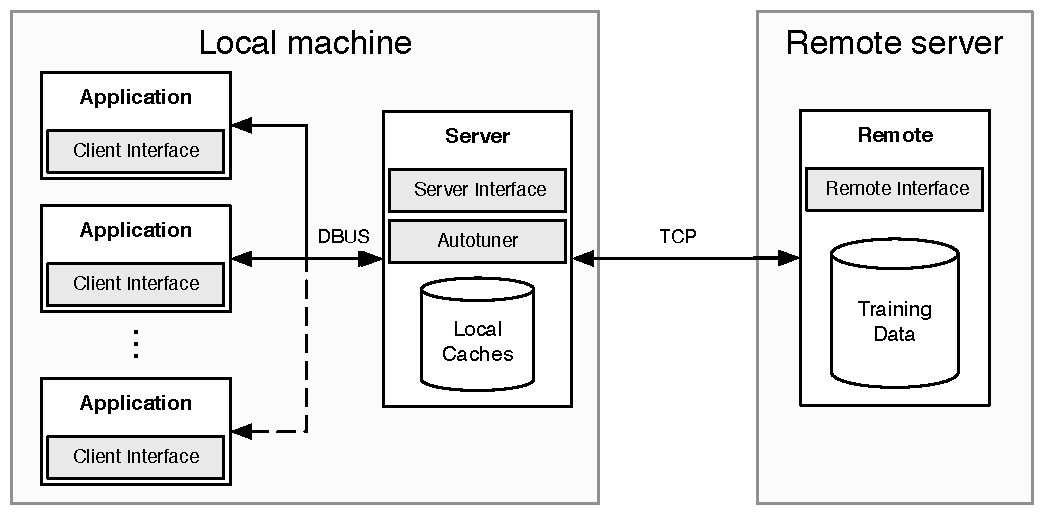
\includegraphics[width=.95\textwidth]{omnitune-system-overview}
\caption{%
  High level system overview of OmniTune.%
}
\label{fig:omnitune-system-overview}
\end{figure}

As discussed in \xref{related work}, common implementations of
autotuning in the literature either: embed the autotuning logic within
the target applications, or take a ``meta-scripting'' approach in
which the autotuner is a standalone program which must be invoked by
the user to tune a target application. The approach taken in this work
aims to capture the advantages of both techniques by implementing an
autotuning service with communication logic embedded in the target
applications. The resulting design consists of three sets of
components: clients, servers, and a global
database. Figure~\ref{fig:omnitune-comms} shows a typical pattern of
communication between the components.

\begin{figure}
\centering
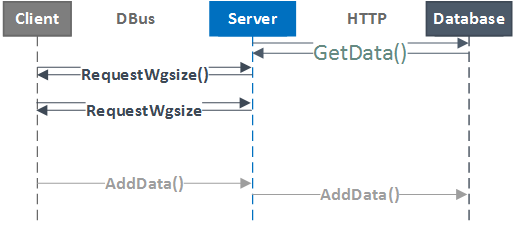
\includegraphics[width=.8\textwidth]{img/omnitune-comms}
\caption{%
  Communication pattern between OmniTune components.%
}
\label{fig:omnitune-comms}
\end{figure}

\TODO{Advantages: asynchronous communication with ``the
  cloud''. Expensive tasks such as model building aren't bound by the
  lifespan of the client application. Lightweight handling of multiple
  connections.}


\subsection{Database: Distributed Training Data}

A master server maintains a common store of all performance
data. \TODO{Write-up schemas, table normal forms, checksum IDs,
  \ldots}


\subsection{Server: Autotuning Engine}

For each autotuning-capable machine, a system-level daemon hosts a
DBus session bus which client processes communicate with. This daemon
acts as an intermediate between the training data and the client
applications, \emph{serving} requests for optimisation parameter
values. The server is implemented as a standalone Python program. On
launch, the server requests the latest training data from the master
database, it then builds the relevant models for performing prediction
of optimisation parameter values. \TODO{Synchronisation, local caching
  and of global DB state.}

OmniTune servers use a plugin system to host proxies that interface
with target applications. Proxies are application-specific, for
example, there is a proxy which implements autotuning of workgroup
size for SkelCL stencils. This proxy exposes two public methods,
\texttt{RequestWgsize} and \texttt{RequestTrainingWgsize}, shown in
Listing~\ref{lst:omnitune-proxy}.

In addition to interfacing with client applications and the database,
OmniTune servers contains a library of generic machine learning tools,
interfacing with Weka\footnote{http://www.cs.waikato.ac.nz/ml/weka/}
using the JNI to perform classification. Each proxy performs feature
extraction of incoming client requests and uses the common machine
learning tools to predict optimal parameter values. \TODO{Plugins
  allow separation of concerns.}

\lstinputlisting[
  language=Python,
  float,
  floatplacement=t,
  label=lst:omnitune-proxy,
  caption={%
    Public OmniTune proxy interface for SkelCL autotuning.%
  }
]{dat/omnitune-skelcl-proxy.py}


\subsection{Client Interface: Lightweight Communication}

By design, the client-server model allows for enabling autotuning with
a low impact on the target applications. As such, the modifications
required to enable OmniTune support within SkelCL were minimal. The
stencil implementation was modified to use an OmniTune client
interface to suggest workgroup sizes, instead of the hardcoded value
which was previously present
(Listing~\ref{lst:skelcl-set-wgsize}). When a SkelCL stencil is
executed, the client interface synchronously calls the
\texttt{RequestWgsize()} method of the OmniTune server, passing as
arguments the required parameters for feature extraction
(Listing~\ref{lst:omnitune-client}). Feature extraction occurs within
the server, which then classifies the extracted features and returns
the suggested workgroup size to the client SkelCL process.

\note{This is a very low latency operation, and the system daemon can
  handle multiple connections from separate SkelCL processes
  simultaneously (although this is an admittedly unlikely use-case
  given that most GPGPU programs expect to be run in isolation).}

\lstinputlisting[
  language=C++,
  float,
  floatplacement=t,
  label=lst:skelcl-set-wgsize,
  caption={
    %
    An extract from the SkelCL stencil implementation, showing the
    call to omnitune client to request workgroup size.
    %
  }
]{dat/skelcl-set-wgsize.cpp}

\lstinputlisting[
  language=C++,
  float,
  floatplacement=t,
  label=lst:omnitune-client,
  caption={
    Implementation of SkeCL's client interface to OmniTune proxy.
  }
]{dat/skelcl-omnitune-client.cpp}


\section{Summary}

This chapter has described the design and implementation of OmniTune,
a distributed autotuner which is capable of performing runtime
prediction of optimal workgroup sizes for SkelCL stencils using a
variety of machine learning approaches. OmniTune uses a client-server
model to decouple the autotuning logic from target programs and to
maintain separation of concerns. It uses lightweight inter-process
communication to achieve low latency autotuning, and uses caches and
lookup tables to minimise the one-off costs of feature
extraction. \TODO{Summarise ML approaches\ldots}
